Early-life exposure to factors associated with poverty is shown to have
adverse long-term effects on labor market outcomes, educational
attainment, and mortality~\citep{Almond_2011}. Hence, many welfare
programs are established to alleviate these effects and help children.
Evidence suggests that parental income is one of the strongest
predictors of one's educational attainment~\citep{Barrow_2012} and
health~\citep{Case_2002}. However, the question of whether cash
transfers to poor families impact children's longevity, educational
attainment, income,~and health is not yet answered.\\
The difficulty in assessing programs as such arises from the many
reasons why cash transfers could potentially fail to help children.
Furthermore, from an evaluation point of view identifying a plausible
counterfactual (i.e.~the outcome in the absence of the treatment) is as
difficult as obtaining data on long-term outcomes. The authors manage to
tackle these difficulties by collecting administrative records from the
Mothers' Pension (MP) program (1911-1935) - the first US
government-sponsored program targeting mothers with dependent children.
As individuals were not eligible for other programs at the time, the
analysis manages to isolate the effect of the unconditional cash
transfers.\\
To investigate the long-term outcomes, the authors track longevity, educational
attainment, health and labor market outcomes of the children of accepted
and rejected applicants. Using the children of mothers who applied and
were deemed eligible but later rejected as a counterfactual, the effect
on longevity was estimated to be approximately a 1-year increase for the
children of accepted mothers. This effect is greater for the poorest
families and very robust to alternative functional form specifications,
alternative counterfactual comparisons, and various treatment of attrition.
Furthermore, to examine the mechanisms through which longevity
increases, different channels are investigated through matching the MP
data with WWII enlistment and 1940 census records. Results yield that
cash transfers reduced the probability of being underweight, increased
educational attainment by 0.34 years, and increased income by 14\%.\\
The analysis excludes females as they are harder to follow, given that
they often change their names after marriage and due to their bad
representation, African-Americans are also not studied. Moreover, the
study suffers from attrition, which is tackled and does not bias the
results.\\
In conclusion, the authors claim that these unconditional cash transfers
manage to improve early life conditions enough to result in better medium- and
long-term outcomes.
\section{Data}\label{data}
\subsection{Mothers' Pension Program}
The MP program is a needs-based program in the US, taking place in 1911
until it is replaced by the Aid to Dependent Children (ADC) in 1935. The
program targets female-headed households, where the breadwinner is
diseased, imprisoned or dead. At the time most of the dependent children
were sent to orphanages and were shown to fare very
poorly~\citep{hopkins2011}. Hence, the main aim of the program was to
provide home care by the mother instead of the child to be sent to an
institution or the mother to be forced into full-time employment. In
terms of size, the program was around 10-30\$ per month, which
represented 29-39\% of maternal income. As the time span and eligibility
differed by state, the average duration of the program was 3 years and
the eligibility is controlled for in the further analysis. All states
required that the mother is poor and the husband is either missing or
incapacitated. The most common cause of discontinuation was remarriage
and therefore, the program should be considered as an unconditional
transfer, rather than being contingent on a specific action by the
recipient.
\subsection{Sample Selection and Matching}
The analysis is limited to males because females are harder to follow
through time due to changing their name after marriage. Furthermore,
more data restrictions are implemented to increase the quality of the
data such as the removal of individuals without dates of birth and with
missing first and/or last name. The working sample from the MP records
contains 16 000 males from 75 counties in 11 states, born
between 1900 and 1925. Of those,~14\% were rejected applicants who
passed a preliminary evaluation but were rejected at a later stage due
to a non-sufficient need of the program. The MP records are then matched
to a Social Security Death Master File (DMF) from 1975 - 2012 in order
to get longevity data. For the analysis of income in adulthood and
educational attainment, the census records from 1940 are used. The data
is further matched with World War II enlistment (WWII) from 1938 - 1946
to account for health outcomes of the children of accepted and rejected
mothers. The problem of attrition is dealth with by assuming that it
is mortality-driven. 48\% of the individuals were matched to a unique
death record, 4\% were matched to multiple death records and 48\% were
not matched. Using live tables, the authors calculate longevity and take
all of the individuals prior to 1975 as death in the follow-up
analysis.
\section{Empirical Strategy and Identification}\label{empirical}
\subsection{Accelerated Failure Time Hazard Model (AFT)}\label{AFT}
The AFT asses the effect of the MP program on the natural logarithm of the age at death for a given individual $i$ in family $f$ born in year $t$, living in county $c$ (state $s$) and has the following functional form:
$$
log(Age\,at\,death)_{ifts} = \theta_0 + \theta_1MP_f + \theta_2\mathbf{X}_{if} + \theta_3\mathbf{Z}_{st} + \mathbf{\theta}_c + \mathbf{\theta}_t + \epsilon_{if}
$$
, where $\theta_1$ is the effect of the program, identified by comparing the average age at death of accepted to rejected boys within county and year of birth, conditional on other observables. $MP_f$ indicates whether the child's mother received MP benefits, $\mathbf{X}_{if}$ is a vector of individual and family characteristics, $\mathbf{Z}_{st}$ represents county-level characteristics in 1910, and state characteristics in the year of application. The authors also control for county fixed effects $\mathbf{\theta}_c$ and cohort fixed effects $\mathbf{\theta}_t$. Standard errors are clustered at the county-level.
\subsection{Survival Regression}\label{probit}
The above specification presents a good overview of the total effect of the program on longevity but fails to deal with attrition and assumes a specific form on the shape of the hazard rate. Hence, the following logit model analyses the probability ($P$) of surviving past age $a$ for a given individual:
$$
P(survived\,to\,age\,a=1)_{iftcs} = f(\theta_0 + \theta_1MP_f + \theta_2\mathbf{X}_{if} + \theta_3\mathbf{Z}_{st} + \mathbf{\theta}_c + \mathbf{\theta}_t + \epsilon_{if})
$$
, where all other covariates are defined as before. The model accounts
for attrition by imputing zero for the unmatched individuals in the DMF
under the assumption that all those without a match were deceased.
Following a comparison between the ``matched sample'' and the
``full-sample'', if the missing data is entirely explained by early
mortality then the full-sample estimates will be correct. To account for
the 4\% multiple matches in the sample, the estimation procedure
by~\citet{Honore_2004} is adopted.
\subsection{Identification}\label{identification}
The identification strategy in this paper uses the children of rejected
but eligible applicants as a counterfactual~\citep{Bound_1989,Wachter_2011}. It relies heavily on the assumption that
accepted and rejected applicants are similar on observable and
unobservable characteristics. This assumption is plausible given the
fact that both groups were aware of the program (unobservable
characteristics) and applied, they were eligible in the beginning and
were probably facing similar economic conditions (observable
characteristics). However, at a later stage, the rejected ones were not
deemed eligible anymore. To investigate this further the authors
performed various tests such as Between-groups comparison; Comparison
of pretreatment characteristics between groups; Examination of reasons
for rejection and discontinuation.\\
The observable characteristics of the two groups look similar but are
not identical. Rejected applicants were on average older and from
smaller families. Furthermore, the exact birth date of accepted
individuals is more likely to be missing, which could be taken as a
marker of illiteracy. The 1915 Iowa census data is then used to assess
whether differences in family characteristics correlate with differences
in family income. After predicting average income for accepted and
rejected applicants by characteristics such as family size, age of
siblings, maternal marital status and length of family name, the
results yield that accepted individuals had 7-9\% lower family income
than rejected. The statistically significant differences between
accepted and rejected applicants at this stage of the analysis
suggest that the accepted mothers came from slightly worse-off
families.\\
The next step involves matching the MP records with two subsamples of
the census data prior to the application in order to obtain information
about pretreatment characteristics. Although these measures are actual
and not predicted they were taken when fathers participated in the
household and not at the time of application when the father is no
longer present. Hence, the measures might not be representative of the
family circumstances at the time of application. Keeping that in mind,
the results are still meaningful and hint that accepted boys come on
average from poorer families.\\
The third step of comparison between the two samples is to examine the
reasons for rejection and discontinuation. By examining the
administrative records, the main reason for rejection was insufficient
need (35\%), marriage or remarriage (8\%), and observed sufficient funds
(as in Clay County, MN and Cook County).\\
All three analyses support the assumption that accepted and rejected
applicants do not differ significantly from each other. The differences
are small and concentrate on the fact that the accepted are slightly
poorer. The analysis proceeds under the assumption that mean
comparisons between these groups represents a lower bound on the effect
of the program.
\section{Mortality Results}\label{results}
\subsection{Main Findings}
Panel A of Table 4 represents the results of the AFT hazard model, where
(1) is a specification based on the sample of individuals with a unique
age at death and only state and cohort dummies, (2) has individual
controls as well as county characteristics in 1910 and state
characteristics at the time of application, (3) adds county fixed
effects. The results are not sensitive to the inclusion of more
controls. In specification (4) the date of birth in the death
certificate is used as opposed to the one in the MP records. In all
specification, the effect of being accepted into the program is
relatively large and positive. Relative to a mean of 72.5 years, the
acceptance increases life expectancy on average with 1.1 - 1.3 years
depending on the specification and sample used.
\begin{figure*}[h!]
\begin{center}
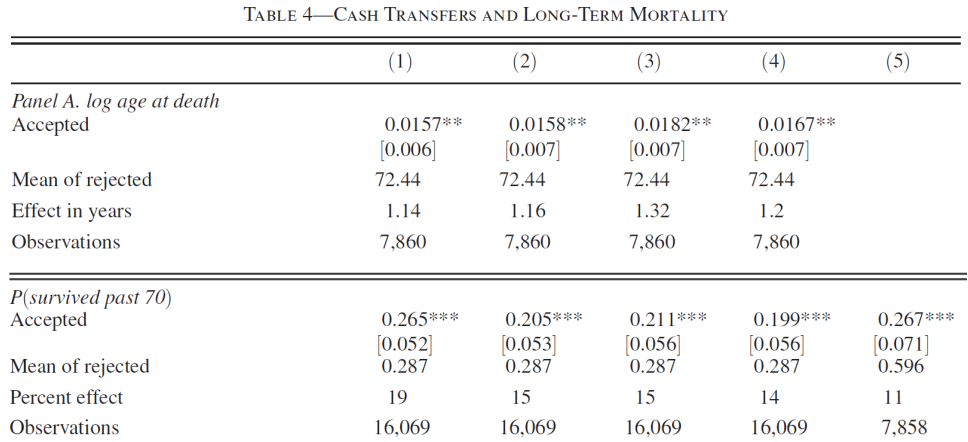
\includegraphics[width=0.98\columnwidth]{table_4_longevity}
\end{center}
\end{figure*}

\noindent
Panel B of Table 4 presents the results from the Logit model. Under the
assumption that those without a match died until the age of 60 ((1)-(4))
and dropping all of them in specification (5), the role of attrition can
be examined. The probability of surviving past the age of 70 increases
significantly for all specifications and is estimated to have a percent
effect of 11-19\%. However, for completeness, the arbitrary cut-offs
are abandoned and Figure 1 shows the estimation of the survival model
using age at death between 58 and 88 (10th and 90th percentiles of the
distribution of the age at death). The marginal effects (as a percentage
of the survival rate of rejected applicants) are computed using the
coefficients from the Logit model. After the age of 67 all of them are
positive and significant in both the full and the matched sample.

\begin{figure}[h!]
\begin{center}
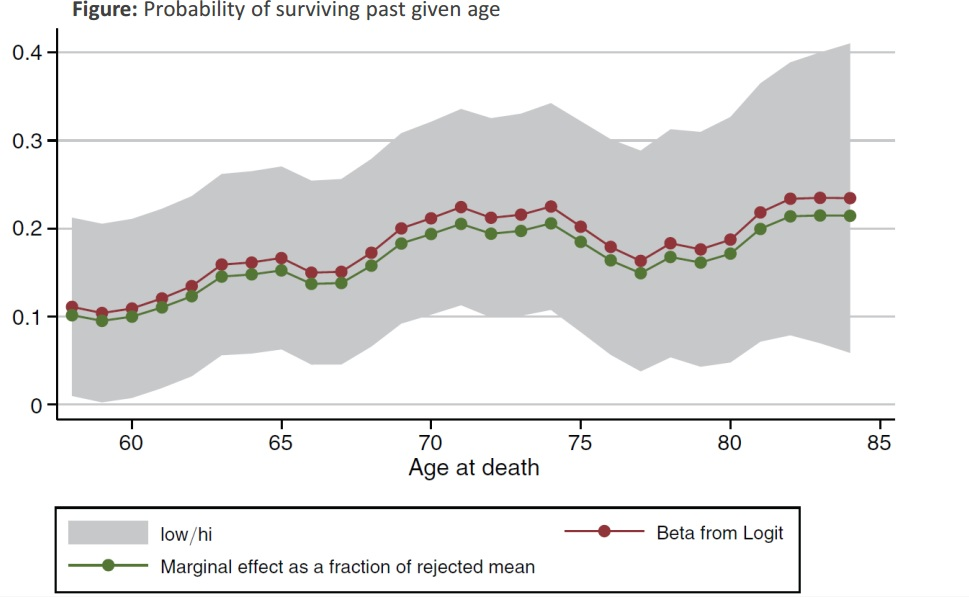
\includegraphics[width=0.84\columnwidth]{figure_1_longevity}
\caption{{Probability of Surviving Past Given Age (Full Sample)
{\label{120529}}%
}}
\end{center}
\end{figure}

\subsection{Robustness Checks}
In order to confirm their results, the authors use various robustness
checks. Here, the specification, the reason they used it and the main
results are briefly mentioned.\\
  \textbf{Heterogeneity by income and urban residence.} By predicting
  family income based on observable demographic characteristics and
  family income in the 1915 Iowa census, the sample is split into low
  income and high income based on deviation from the median predicted
  income. Comparing rejected and accepted families across the two groups
  yields 15\% higher increase in longevity for the low income
  individuals compared to the high income ones (not statistically
  significant results). After splitting into 3 groups by child age,
  larger but not statistically significant results are found for younger
  children. Furthermore, the residential area is put under
  investigation, given the fact that counties had the administrative
  power in the MP program. Splitting the sample into above and below
  median share urban, no significant difference in size is observed
  between the two samples. Hence, there are not statistically significant deviations from the original results. However, the effects are assumed to be stronger for poorer families.\\
  \textbf{Discrimination and the composition of rejected applicants.} To
  test their identification strategy, the authors examine if there are
  unobservable characteristics such as race and nativity, that can
  negatively correlate with children outcomes through discrimination.
  Although the US Department of Labor estimated that 96\% of the MP
  recipients were white, linking a subset of the records with WWII
  enlistment and 1940 census data that contain race did not show that
  blacks were more likely to be rejected. Furthermore, the Department of
  Labor reposted lack of discrimination in 1931 for Ohio. Discrimination
  towards nativity was also not found, however, there exist
  contradictory reports arguing each side. Matching with different
  sources for finding nativity and dropping individuals subsequently by
  age of the child, family size does not suggest any type of different
  treatment between the groups. Therefore, discrimination is not considered to bias the results.\\
  \textbf{Aggregate results.} Estimated models with aggregated data on
  county level, year of application and year of birth by regressing the
  fraction surviving past age 70 on fraction accepted did not yield
  significantly different results whether using weights or controls.
  This robustness check excludes the possibility of counties with high
  rejection rates driving the results.\\
  \textbf{Results for Ohio.} Since 34\% of the sample originates from
  Ohio, where black mothers received benefits at expected rates, the
  applicants were not required to be U.S~citizens, and there is
  availability of data on other social programs taking place at the same
  time. Results remain robust but slightly larger. Hence, discrimination
  and availability of other programs are not biasing the results.\\
  \textbf{Attrition and multiple matches.} Given the different rate of
  attrition between rejected and accepted applicants (51\% vs. 45\%
  respectively), the authors want to show that this is due to mortality
  rather than other factors. Further analysis on the lifetables shows
  that the magnitude of the attrition is consistent with the magnitude
  of the mortality rates. Matching with retrospective pre-application
  records indicates that differences in the names of accepted and
  rejected applicants do not have an effect on the match rate. Lastly,
  the rate of multiple matches is the same across the two samples.
  Additional death records are collected for the state of Ohio, where
  further analysis shows that the rejected applicants did die younger
  than the accepted ones, which confirms the assumption that the
  difference in the matching rates is due to mortality. The results are
  also not sensitive to the treatment of multiple matches. Therefore, this robustness check supports the assumption that attrition is mortality driven. \\
  \textbf{Alternative counterfactulas.} Two alternative control groups
  are constructed from 1900, 1910, 1920, and 1930 census matched with
  their DMF records. Orphans - children living in institutions are an
  appropriate historical counterfactual as one of the purposes of the MP
  program is to prevent the institutionalization of children. This group
  is very similar to rejected applicants with regard to longevity,
  confirming the findings that they live shorter lives than accepted
  applicants. The second control group considered here are single or
  divorced mothers, not eligible for the MP program according to the
  laws of some states. Comparing these children to children whose
  fathers were disabled or institutionalized found the same results as
  the main analysis. Children of accepted mothers lived longer compared
  to the control group.\\
All robustness checks support the original findings and hence,
strengthen the reliability of the paper.
\section{Income, Educational Attainment, and Health Results}\label{other results}
To examine the mechanisms through which longevity is increased by income
transfers in the childhood, the authors focus on factors associated with
mortality. Such factors are education, income, and
weight~\citep{Flegal_2005, Cutler_2006, Deaton_2001}.
These possible medium-term adulthood outcomes are examined by merging
with the 1940 census records and Worl War II enlistment records.
\subsection{Income and Educational Attainment}
As it can be seen in Panel A of Figure 2, the income distribution is
shifted to the right for accepted boys. The regression results suggest that boys of
MP recipients have 14\% higher incomes in 1940. Additionally, the
accepted boys were more likely to have graduated highschool and results
on average in 0.3 - 0.4 more years of schooling (Panel B, Figure 2).
\begin{figure}[h!]
\begin{center}
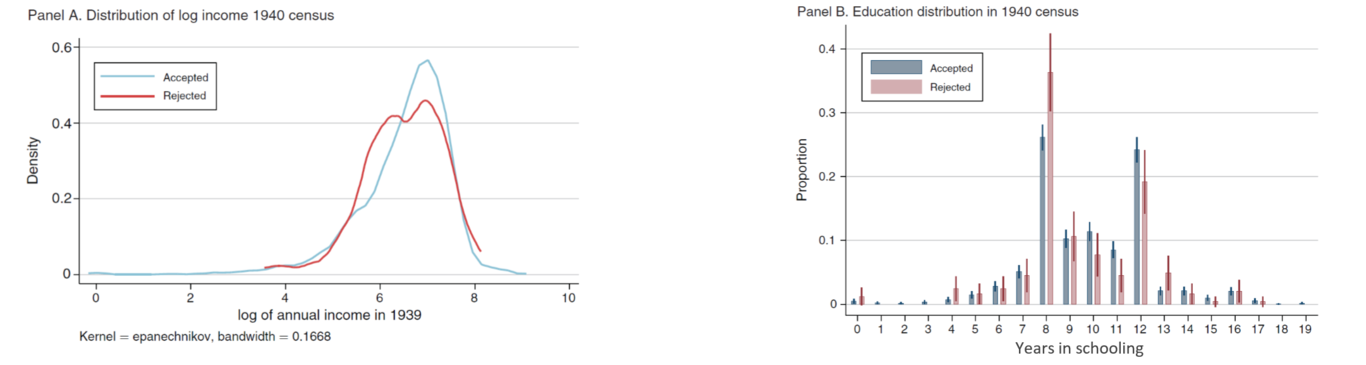
\includegraphics[width=1.00\columnwidth]{figure_2_income_education}
\caption{{Income and Education Results
}}
\end{center}
\end{figure}
\subsection{Health}
To obtain health results, a subsample of the MP records has to be
matched with their WWII enlistment records for the cohort that enlisted
the Army during 1938-1946. However, the match rate to the records is
rather low (17.2\% of males overall) since they do not contain
exact date of birth. Furthermore, it has to be noted that participants
in the enlistment are a selected subsample of the population because of
induction rules and exemptions, hence, they are on average younger,
healthier, and more highly educated. Table 7 reports that the
participation in the MP program suggests a significant reduction in the
probability of being underweight. The estimates for height, weight,~and
BMI are also positive, concluding that the accepted families managed to
improve the nutrition of their children.
\begin{figure*}[h!]
\begin{center}
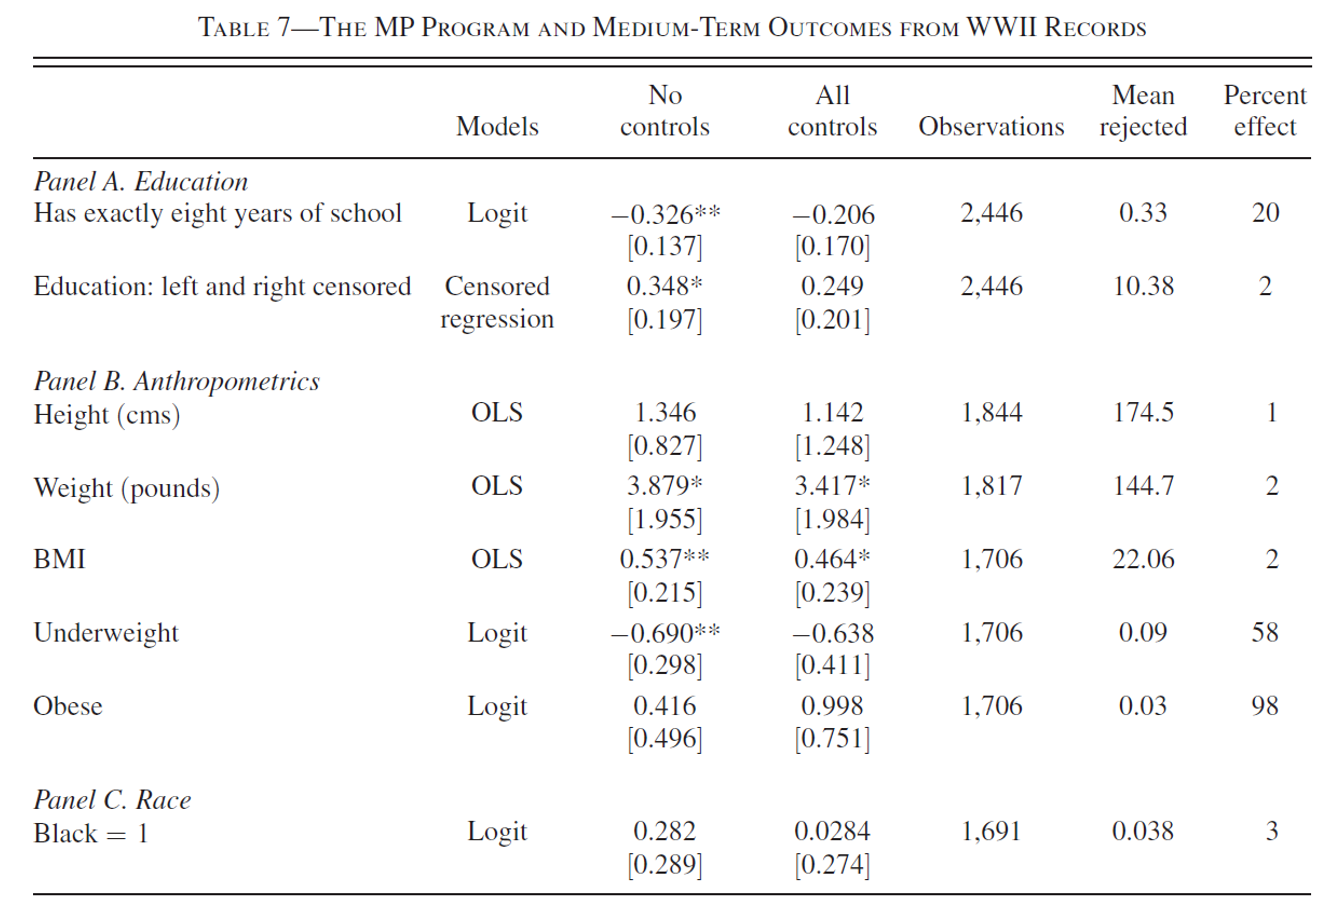
\includegraphics[width=0.98\columnwidth]{table_7_health}
\end{center}
\end{figure*}
The expected decrease in mortality through the channel of malnutrition
is rather small, given the fact that only 10\% of the subsample is
underweight, although the overall effect is big in size considering the
relative risk of mortality ranges from 1.38 to
2.3. Looking at the estimates of education and income, they have
higher explanatory power in this particular situation. That suggests a
30\% increase in income would lower mortality by 10\%, increasing
longevity by 0.9 years. Moreover, an increase in schooling of 0.25 years
is associated with a 0.15 years increase in longevity. In conclusion,
participation in the MP program would result in at least one additional
year of longevity, consistent with the previous results from Table 4 of
1.1-1.4 years. Which leads to these mechanisms explaining 75-95 \% of
the increase in life expectancy.
\section{Interpretation and Policy Relevance}
The study finds that participation in the MP program increases
longevity, possibly through the mechanisms examined in the paper:
income, education, and health. The results depend heavily on the
counterfactual chosen for the study. The findings are supported by the
various robustness checks and are deemed relevant despite the different
conditions in the twenty-first century. Namely, single mothers are still
representative of the poorest families. Parental income has similar
implications on children's human capital and the estimates for short-
and medium-term effects are consistent with other work.
\section{Critical Assessment}
\textbf{Strengths and Contribution:} Strong identification. Data on long-term outcomes. Various robustness checks supporting the initial results. Papers where the paper is in line with the literature on short and medium- run outcomes.\\
\textbf{Main Assumptions:} Attrition via mortality. The accepted and rejected are the same. \\
\textbf{Effects sizes:} Possible underestimation of the effect because of positive
externality from the accepted to the rejected in terms of health. Possible overestimation of the increase in income, through the
channel of other programs, benefiting the rejected applicants.\\
\textbf{External Validity and Effectiveness:} External validity to today's world: Women have more labor market
opportunities today; Conditions without transfers might differ today;
Families receiving cash assistance today could have changed their
behavior. Effectiveness: Receivers might not maximize their children's
well-being with the additional money; the money might not be sufficient
to drive such results.